\chapter{Experiments and Results}
\label{section:analysis}

\section{Scenarios}
Several different scenarios are used to test the algorithm. Each scenario takes place in a world with a certain distribution of obstacles, has a start and goal position, and a UAV with certain characteristics.
\par
There are three categories of scenarios, which will be discussed in section \ref{subsec:synth} to \ref{subsec:leuven}. All scenarios are tested in a general performance test (section \ref{subsec:gen-perf}) to get an overview of the performance of the algorithm with the default parameters. This test determines whether or not the algorithm scales to large and complex environments.\\
In the other tests, only one scenario of each category has been used. Section \ref{subsec:agility} tests the performance of the algorithm as the characteristics of the UAV change. Section \ref{subsec:stability} looks at the stability of the algorithm. These tests should provide further insight on the limitations of the algorithm.\\

Sections \ref{subsec:cutting} to \ref{subsec:approach-margin} look at the effects of different parameters on both the performance of the algorithm and the quality of the trajectory. Sensible default parameters have been chosen. However, changing these parameters provides deeper insights in the characteristics of the algorithm.

All tests were executed on an Intel Core i5-4690k running at 4.4GHz with 16GB of 1600MHz DDR3 memory. The reported times are averages of 5 runs, unless stated otherwise. The machine runs on Windows 10 using version 12.6 of IBM CPLEX. Table \ref{table:params} show the default parameters as used in all tests.

\begin{figure}[h]
\centering
\begin{tabular}{ l  r | l r }
grid size 			& $2m$ 	& turn tolerance 		& $2$ \\
approach multiplier & $2$ 	& population size 		& $ 10$ \\
\# generations 		& $25$ 	& max. nudge distance 	& $5m$\\
min. \# vertices 	& $ 4$ 	& max. \# vertices 		& $12$ \\
P(add vertex) 		& $0.1$ & P(remove vertex) 		& $0.1$  \\
max nudge attempts 	& $15$ 	& $ T_{max}$ 			& $5s$ \\
time step size 		& $0.2s$& position tolerance & $3$ \\
CPLEX max solve time & $120s$ & CPLEX max delta & $1$ \\
time limit multiplier & $1.5$ & max segment time & $3s$\\
linear approx vertices & $12$ & & \\
%approach margin, maxsegment time
%fps
%pop, gens, mutrate, nudge dist, minpoints-maxpoints, addprob, removeprob
\end{tabular}
\caption{The parameters used for testing}
\label{table:params}
\end{figure}
\clearpage
\subsection{Synthetic Scenarios}
\label{subsec:synth}
The synthetic scenarios have small, handmade worlds. They have few obstacles, but the obstacles are laid out in a way that makes them challenging to solve. There are two "Up/Down" scenarios, small (Figure \ref{fig:bench-small}) and large (Figure \ref{fig:bench-large}), in which the UAV has to move in a zig-zag pattern to reach its goal. The difference between those scenarios is the amount of obstacles, which also changes the amount of zig-zags required. These scenarios are built to see how the algorithm handles sharp turns. There is also a spiral scenario in which the UAV must go in an outwards spiral (Figure \ref{fig:spiral}.\\
The large Up/Down scenario represents this category in the tests. Table \ref{table:uav-synth} shows the properties of the UAV.

\begin{table}[h]
\centering
\begin{tabular}{ c | c | c }
$v_{max}$ ($ms^{-1}$)	& $a_{max}$ ($ms^{-2}$) 	& radius ($m$) 	 \\
\hline
$3$ & $4$ 	& $0.5$ \\
\end{tabular}
\caption{The UAV properties for the synthetic scenarios}
\label{table:uav-synth}
\end{table}

\begin{figure}
	\centering
	
	\begin{subfigure}[t]{0.5\textwidth}
        		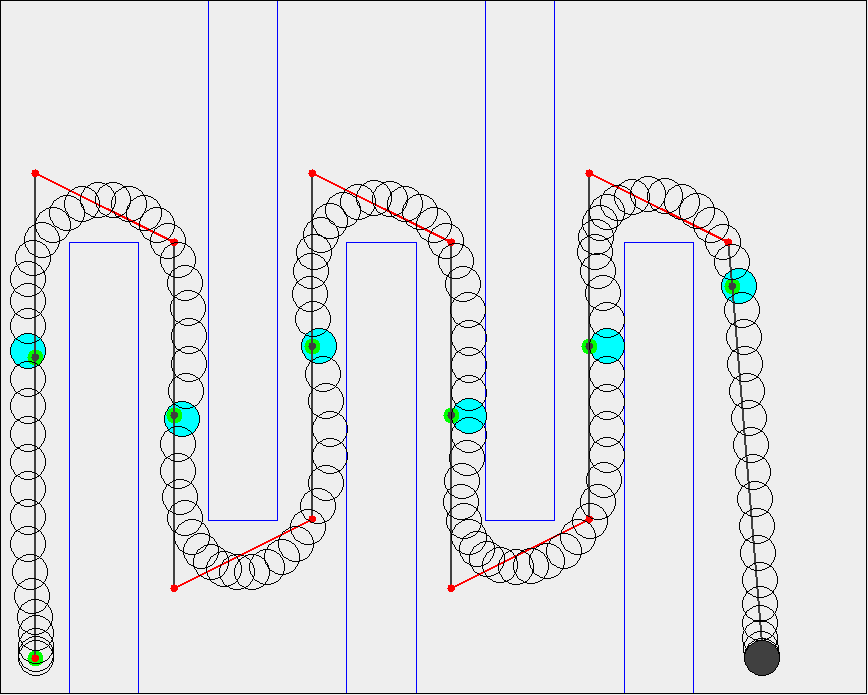
\includegraphics[width=\textwidth]{img/bench-small}
        		\caption{}
        		\label{fig:bench-small}
	\end{subfigure}
		
	\begin{subfigure}[t]{0.6\textwidth}
        		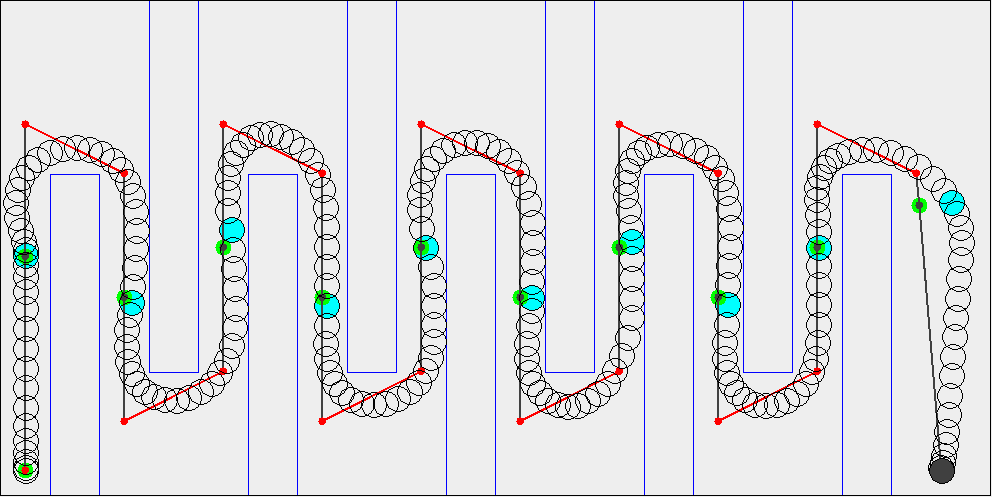
\includegraphics[width=\textwidth]{img/bench-large}
        		\caption{}
        		\label{fig:bench-large}
	\end{subfigure}	
	
	\begin{subfigure}[t]{0.5\textwidth}
        		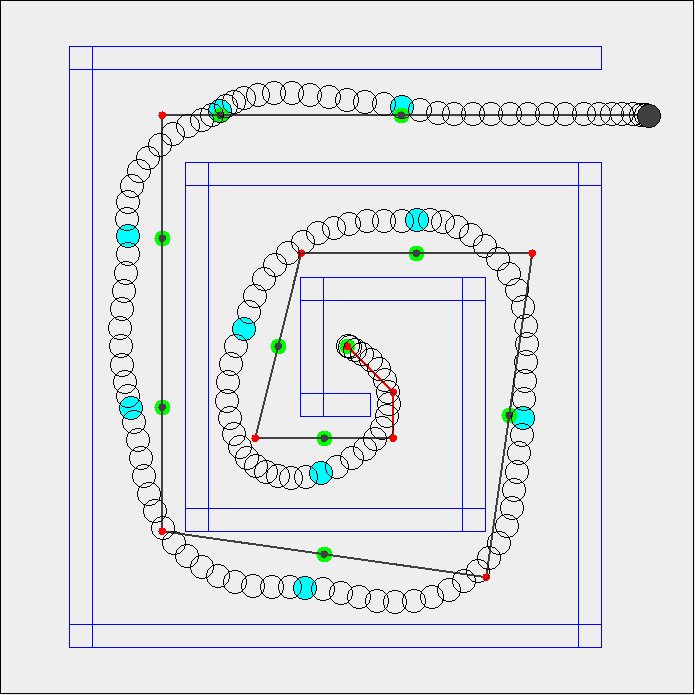
\includegraphics[width=\textwidth]{img/spiral}
        		\caption{}
        		\label{fig:spiral}
	\end{subfigure}
        
    \caption{The synthetic scenarios}\label{fig:synth-scens}
\end{figure}
\clearpage
\subsection{San Francisco Scenarios}
\label{subsec:sf}
The San Francisco scenarios contain a world which is based on a map of San Francisco. There are 2 small San Francisco scenarios (Figure \ref{fig:sf-small-1} and \ref{fig:sf-small-2}), which both share the same 1km by 1km area of San Francisco but have different start and goal locations. There is also a larger San Francisco scenario which takes places on a 3km by 3km world (Figure \ref{fig:sf-large}). \\
All obstacles in the San Francisco dataset are grid-aligned rectangles, laid out in typical city blocks. Because of this, density of obstacles is predictable. These scenarios showcase that the algorithm can scale to realistic scenarios with much more obstacles than is typically possible with a MILP approach. \\
The first small San Francisco scenario is used to represent this category in the tests. Table \ref{table:uav-sf} shows the properties of the UAV and Figure \ref{fig:sf-zoom} shows a zoomed-in view of the first small scenario. 


\begin{table}[h]
\centering
\begin{tabular}{ c | c | c }
$v_{max}$ ($ms^{-1}$)	& $a_{max}$ ($ms^{-2}$) 	& radius ($m$) 	 \\
\hline
$10$ & $15$ 	& $2.5$ \\
\end{tabular}
\caption{The UAV properties for the San Francisco scenarios}
\label{table:uav-sf}
\end{table}

\begin{figure}[h]
	\centering
	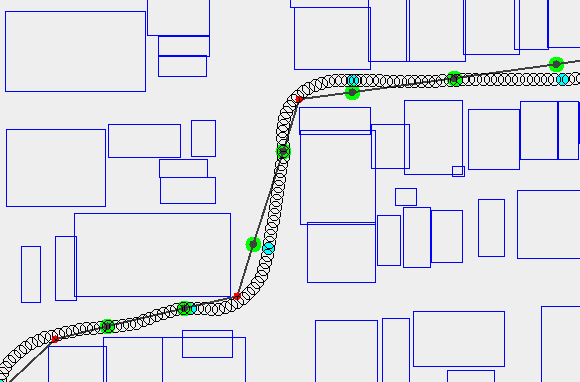
\includegraphics[width=0.8\textwidth]{sf-zoom}
	\caption{A zoomed-in view of the first small the San Francisco scenario}
	\label{fig:sf-zoom}
\end{figure}


\begin{figure}
	\centering
	
	\begin{subfigure}[t]{0.46\textwidth}
        		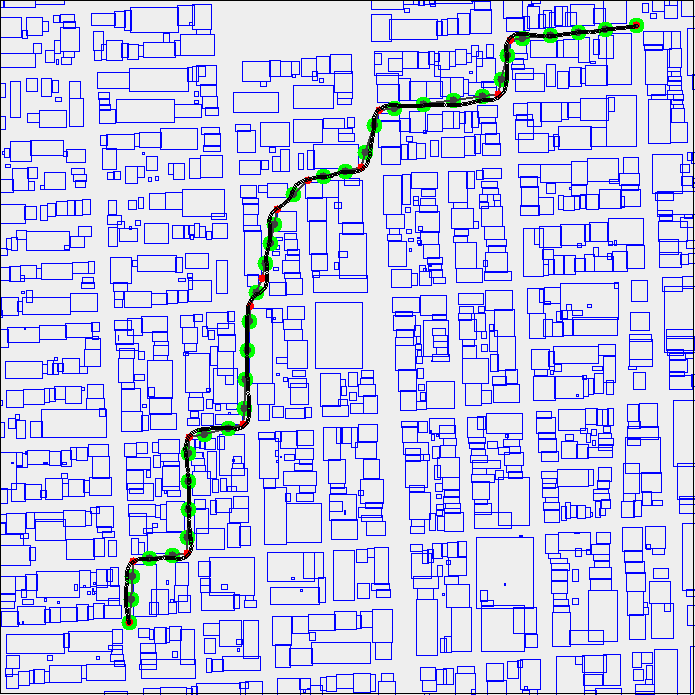
\includegraphics[width=\textwidth]{img/sf-small-1}
        		\caption{San Francisco Small 1}
        		\label{fig:sf-small-1}
	\end{subfigure}
	\hfil	
	\begin{subfigure}[t]{0.46\textwidth}
        		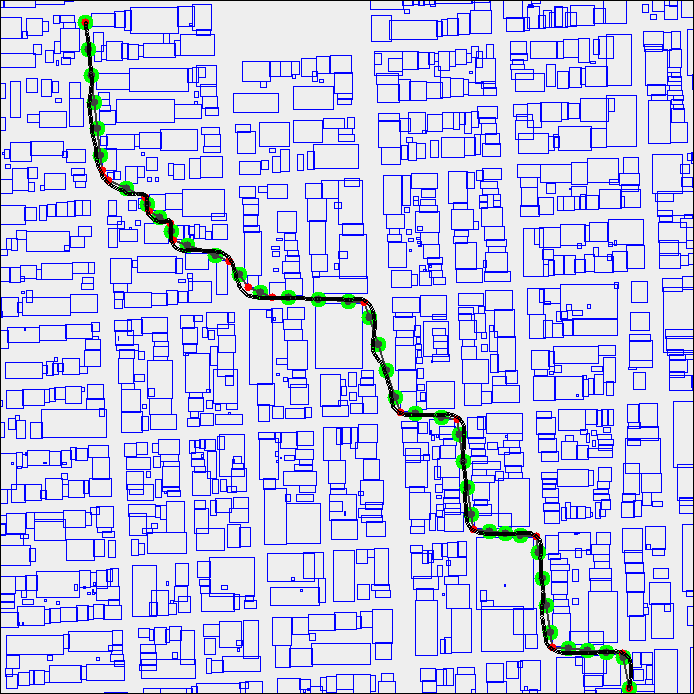
\includegraphics[width=\textwidth]{img/sf-small-2}
        		\caption{San Francisco Small 2}
        		\label{fig:sf-small-2}
	\end{subfigure}	
	\par
	\begin{subfigure}[t]{0.8\textwidth}
        		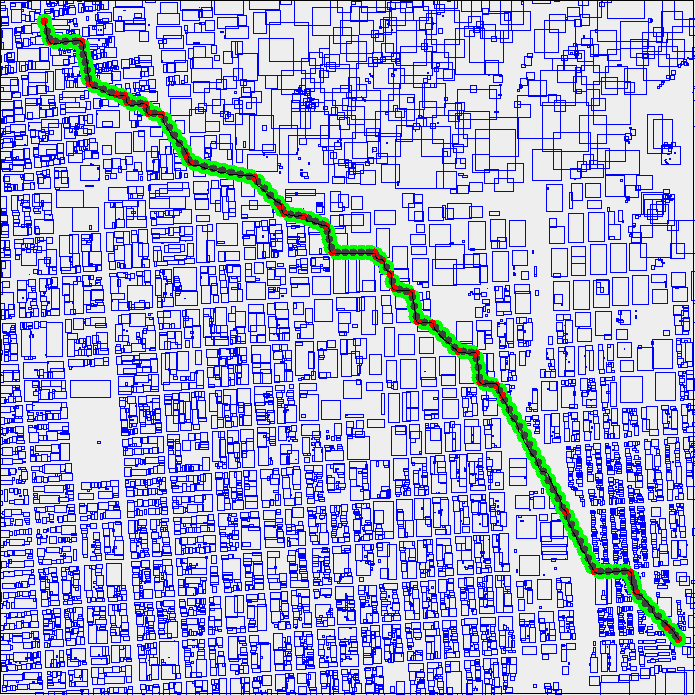
\includegraphics[width=\textwidth]{img/sf-large}
        		\caption{San Francisco Large}
        		\label{fig:sf-large}
	\end{subfigure}
        
    \caption{The San Francisco scenarios}\label{fig:sf-scens}
\end{figure}

\clearpage
\subsection{Leuven Scenario}
\label{subsec:leuven}
The Leuven scenarios contain a world based on a map of the city of Leuven. This is an old city with a very irregular layout. The dataset, provided by the local government\footnote{\url{https://overheid.vlaanderen.be/producten-diensten/basiskaart-vlaanderen-grb}}, also contains full polygons instead of the grid-aligned rectangles of the San Francisco dataset. While most buildings in the city are low enough so a UAV could fly over, it presents a very difficult test case for the path planning algorithm. The density of obstacles varies greatly and is much higher than in the San Francisco dataset across the board.\\
The first small Leuven scenario is used to represent this category in the tests. Table \ref{table:uav-leuven} shows the properties of the UAV and Figure \ref{fig:leuven-zoom} shows a zoomed-in view of the first small scenario. 
\begin{table}[h]
\centering
\begin{tabular}{ c | c | c }
$v_{max}$ ($ms^{-1}$)	& $a_{max}$ ($ms^{-2}$) 	& radius ($m$) 	 \\
\hline
$10$ & $15$ 	& $1$ \\
\end{tabular}
\caption{The UAV properties for the Leuven scenarios}
\label{table:uav-leuven}
\end{table}

\begin{figure}[h]
	\centering
	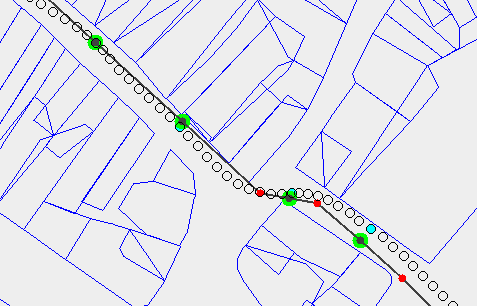
\includegraphics[width=0.8\textwidth]{leuven-zoom}
	\caption{A zoomed-in view of the first small the Leuven scenario}
	\label{fig:sf-zoom}
\end{figure}



\begin{figure}
	\centering
	
	\begin{subfigure}[t]{0.46\textwidth}
        		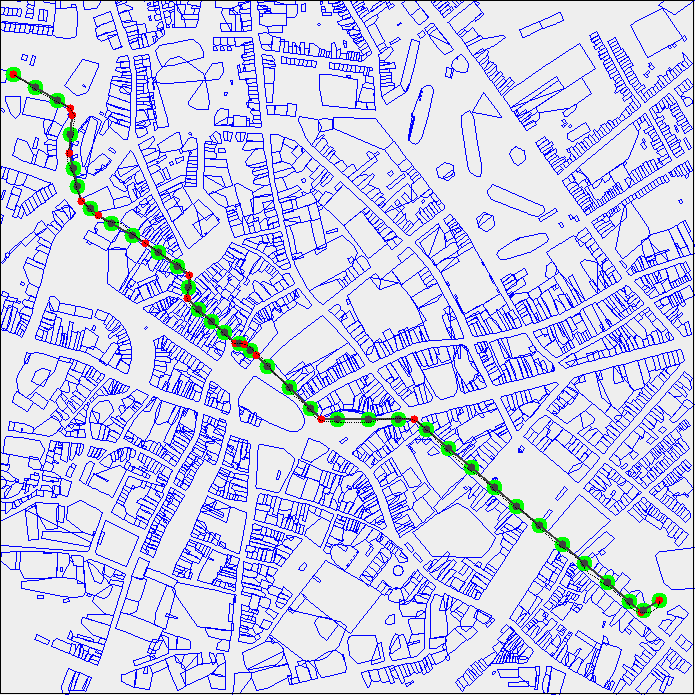
\includegraphics[width=\textwidth]{img/leuven-small-1}
        		\caption{Leuven Small 1}
        		\label{fig:leuven-small-1}
	\end{subfigure}
	\hfil	
	\begin{subfigure}[t]{0.46\textwidth}
        		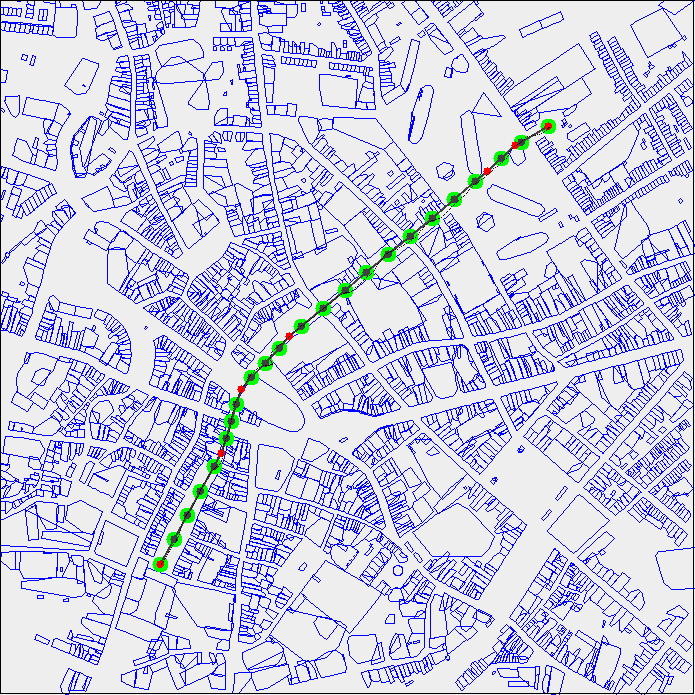
\includegraphics[width=\textwidth]{img/leuven-small-2}
        		\caption{Leuven Small 2}
        		\label{fig:leuven-small-2}
	\end{subfigure}	
	\par
	\begin{subfigure}[t]{0.8\textwidth}
        		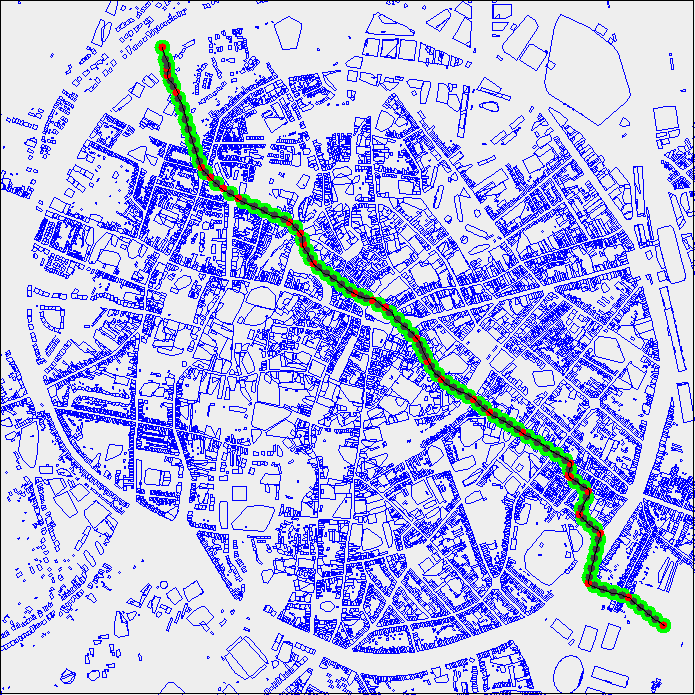
\includegraphics[width=\textwidth]{img/leuven-large}
        		\caption{Leuven Large}
        		\label{fig:leuven-large}
	\end{subfigure}
        
    \caption{The Leuven scenarios}\label{fig:sf-scens}
\end{figure}
\clearpage
\section{General Performance}
In this test, the general performance of the different parts of the algorithm are tested. Every scenario is tested with the default parameters. Table \ref{table:gen-data} shows some detailed information about the scenarios, including the length of the Theta* path and the amount of segments problem is divided into. Table \ref{table:gen-results} shows the execution parts for the most computationally expensive parts of the algorithm (the Theta* path, genetic algorithm and MILP solver), as well as the total time required. It also shows the score of the resulting trajectories. This score is in seconds and is the amount of time that the UAV needs to reach the goal position when following the trajectory. 

\label{subsec:gen-perf}
\begin{table}[]
\centering
\begin{tabular}{ l | r | l | r | r}
Scenario name & \# obstacles & world size & path length (m)  & \# segments \\
\hline
Up/Down Small 	& 5 	& 25m x 20m 	& 88 	& 7   \\ 
Up/Down Large 	& 9 	& 40m x 20m 	& 146 	& 11  \\
Spiral		 	& 11 	& 30m x 30m 	& 96 	& 10  \\
SF Small 1		& 684 	& 1km x 1km 	& 1392 	& 34  \\
SF Small 2		& 684 	& 1km x 1km 	& 1490 	& 38  \\
SF Large	 	& 6580 	& 3km x 3km 	& 4325 	& 107 \\
Leuven Small 1 	& 3079 	& 1km x 1km 	& 1312 	& 34  \\
Leuven Small 2	& 3079 	& 1km x 1km 	& 864 	& 22  \\
Leuven Large 	& 18876	& 3km x 3km 	& 3041 	& 78  \\
\end{tabular}
\caption{Some information about the scenarios tested.}
\label{table:gen-data}
\end{table}

\begin{table}[]
\centering
\begin{tabular}{ l | r | r | r | r || r}
Scenario name & Theta* (s) & GA (s) & MILP (s)  & total (s) & score (s) \\
\hline
Up/Down Small 	& 0.00 	& 0.33 	& 10.48 & 10.97 & 27.24	\\ 
Up/Down Large 	& 0.00 	& 0.65 	& 17.95 & 18.87 & 44.76	\\
Spiral		 	& 0.01 	& 1.06	& 7.17	& 8.46 	& 28.72	\\
SF Small 1		& 1.37 	& 7.68 	& 32.81 & 42.43 & 106.20\\
SF Small 2		& 1.82 	& 7.98	& 36.81 & 47.32 & 114.36\\
SF Large	 	& 15.88	& 15.41	& 75.44 & 108.28 & 325.10\\
Leuven Small 1 	& 1.51 	& 23.49	& 135.86& 161.85& 97.44	\\
Leuven Small 2	& 0.53 	& 14.00	& 62.03 & 76.99 & 65.52	\\
Leuven Large 	& 14.65	& 67.55	& 460.46 & 544.73 & 227.27\\
\end{tabular}
\caption{A breakdown of the execution time for each scenario, as well as the score of the trajectory.}
\label{table:gen-results}
\end{table}


\begin{figure}
	\centering
	
	\begin{subfigure}[t]{.40\textwidth}
        		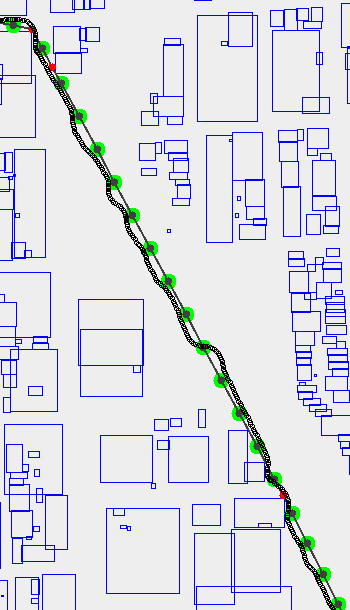
\includegraphics[width=\textwidth]{img/sf-sparse}
        		\caption{The large San Francisco scenario has a region with very sparse obstacles.}
        		\label{fig:sf-sparse}
	\end{subfigure}
	\hfil
	\begin{subfigure}[t]{.45\textwidth}
        		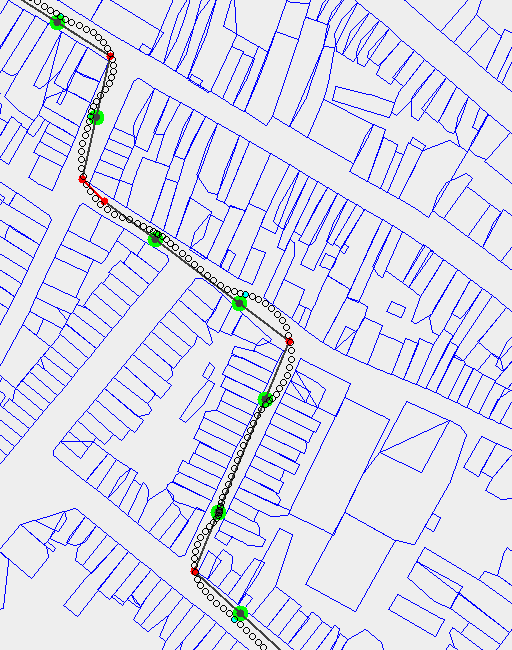
\includegraphics[width=\textwidth]{img/leuven-dense-2}
        		\caption{The large Leuven scenario passes through several regions with very dense obstacles}
        		\label{fig:leuven-dense}
	\end{subfigure}	
	
        
    \caption{}\label{fig:perf-density}
\end{figure}



\begin{table}[]
\centering
\begin{tabular}{ l | r | r | r | r | r}
Scenario name & path length(m) & Theta* (s) & GA (s) & MILP (s)  & total (s) \\
\hline
Up/Down Small 	& 12.57	& 0.00 	& 0.05 	& 1.50 	& 1.57 	\\ 
Up/Down Large 	& 13.27	& 0.00 	& 0.06 	& 1.63 	& 1.72 	\\
Spiral		 	& 9.60	& 0.00 	& 0.11	& 0.72	& 0.85	\\
SF Small 1		& 40.94 & 0.04 	& 0.23 	& 0.97 	& 1.25 	\\
SF Small 2		& 39.21	& 0.05 	& 0.21	& 0.97 	& 1.25 	\\
SF Large	 	& 40.42	& 0.15	& 0.14	& 0.71 	& 1.01 	\\
Leuven Small 1 	& 38.59	& 0.04 	& 0.69	& 4.00	& 4.76	\\
Leuven Small 2	& 39.27	& 0.02 	& 0.64	& 2.82 	& 3.50	\\
Leuven Large 	& 38.99	& 0.19	& 0.87	& 5.9 	& 6.98 	\\
\end{tabular}
\caption{A breakdown of the execution time per segment}
\label{table:gen-results-rel}
\end{table}


\subsection{Interpretation}
With the default settings, the algorithm is capable of solving all scenarios within a reasonable amount of time. In every case, solving the MILP problem takes the majority of the time. \\
The amount of segments differs between these scenarios. Table \ref{table:gen-results-rel} expresses the results relative to the amount of segments, as well as the path length per segment.
\par
A first observation is that the path length per segment is very similar for all San Francisco and Leuven segment. The UAV has the same maximum velocity and acceleration in those scenarios. Even though the density and layout of the obstacles is very different, the amount of segments scales linearly with the path length as long as the UAV properties remain the same.
\par
Another observation is that the relative time needed to calculate the Theta* path increases as the path length increases. This is not surprising since Theta*, like A*, has an exponential worst-case complexity. This means that the scalability of Theta* puts an upper limit on the scalability of the entire algorithm.
\par
The next observation is the genetic algorithm (GA) execution time and MILP solve times are very similar within categories. For the synthetic category, the Up/Down scenarios are virtually identical in both measures. The spiral scenario is hard to compare since it is very different.  \\
For the San Francisco scenarios, the two small scenarios have very similar GA and MILP execution times, but the larger scenario comes in lower. The two small Leuven scenarios are also similar in GA execution time, although the first scenario has a higher MILP solve time. The large Leuven scenario has higher execution times for both the GA and MILP solver.
\par
These variations can be explained by differences in densities between the scenarios. In the large San Francisco scenario, the trajectory crosses a region with very sparse buildings (Figure \ref{fig:sf-sparse}). The sections in the regions are easier to solve than in the smaller scenarios. The opposite happens in the large Leuven scenario, which passes through several regions with very dense obstacles (Figure \ref{fig:leuven-dense}). These account for the significant increase in execution time for both the genetic algorithm as the MILP solver.


\clearpage
\section{Agility of the UAV}
\label{subsec:agility}
The properties of the segments strongly rely on the agility of the UAV. The size of the segments is determined by the maximum acceleration distance of the UAV. \\
This experiment tests the relation between the maximum velocity and the maximum acceleration of the UAV. This test was executed on the standard set of scenarios: the large Up/Down scenario, the small San Francisco scenario and the small Leuven scenario. For each scenario I tested nine configurations of the vehicle: Every combination between three different maximum velocities and three different maximum accelerations. Table \ref{table:synth-agility} shows the different UAV properties for the Up/Down scenario, Table \ref{table:sf-leuven-agility} shows the same properties for the San Francisco and Leuven Scenarios. Table \ref{table:synth-agility-data}, \ref{table:sf-agility-data} and \ref{table:leuven-agility-data} shows the results for respectively the Up/Down, San Francisco and Leuven scenarios. Figure \ref{fig:agility-low}, \ref{fig:agility-med} and \ref{fig:agility-high} show the same data, but fix either the acceleration or velocity and vary the other property. \\

\begin{table}[h]
\centering
\begin{tabular}{ c || c | c | c}
 & Low & Med & High \\
\hline\hline
Velocity ($ms^{-1}$) 	& 2		& 4		& 8 	\\ 
\hline
Acceleration ($ms^{-2}$)& 1		& 3 	& 6 	\\  
\end{tabular}
\caption{The different maximum velocity and acceleration values for the vehicle for the Up/Down scenario.}
\label{table:synth-agility}
\end{table}

\begin{table}[h]
\centering
\begin{tabular}{ c || c | c | c}
 & Low & Med & High \\
\hline\hline
Velocity ($ms^{-1}$) 	& 5		& 15	& 30 	\\ 
\hline
Acceleration ($ms^{-2}$)& 3		& 10	& 20 	\\  
\end{tabular}
\caption{The different maximum velocity and acceleration values for the vehicle for the San Francisco and Leuven scenarios.}
\label{table:sf-leuven-agility}
\end{table}

\clearpage

\begin{table}[]
\centering
\begin{tabular}{ c || r | r | r}
solve time (s) & Low vel& Med vel& High vel\\
\hline\hline
Low acc 	& 26.08		& 91.98		& 100.28	\\ \hline
Med acc		& 9.93		& 16.93		& 15.17		\\  \hline
High acc	& 7.23		& 6.39		& 4.85 		\\  
\end{tabular}
\caption{Up/Down}
\label{table:synth-agility-data}
\end{table}

\begin{table}[]
\centering
\begin{tabular}{ c || r | r | r}
solve time (s) & Low vel& Med vel& High vel\\
\hline\hline
Low acc 	& 57.3		& -			& -			\\ \hline
Med acc		& 22.78		& 31.85		& 483.17	\\  \hline
High acc	& 19.53		& 13.75		& 39.64 		\\  
\end{tabular}
\caption{San Francisco}
\label{table:sf-agility-data}
\end{table}


\begin{table}[]
\centering
\begin{tabular}{ c || r | r | r}
solve time (s) & Low vel& Med vel& High vel\\
\hline\hline
Low acc 	& 127.62	& -			& -			\\ \hline
Med acc		& 64.16		& 118.86	& -			\\  \hline
High acc	& 60.83		& 53.8		& - 		\\  
\end{tabular}
\caption{Leuvem}
\label{table:leuven-agility-data}
\end{table}

\subsection{Interpretation}
Several of the combinations failed to complete because the segments could not be solved within 120 seconds each. The general trend is that a higher maximum acceleration and a lower maximum velocity decrease the solve time. This is as expected, as both of those make the maximum acceleration distance smaller. A larger maximum acceleration distance leads to larger segments with more obstacles in them, which have a negative effect on the performance. 
\par
When the acceleration is high, varying the velocity has an unexpected effect. When going from a low to medium maximum velocity, the solve time actually decreases for all scenarios. I do not have an explanation for why this happens.
\par
Another slightly unexpected result is that the combination of a high maximum acceleration and high maximum velocity fails for the Leuven scenario. This is not a particularly difficult combination for the other scenarios, so the failure is unexpected.
\par
The default UAV properties seem to be right on the limit for the Leuven scenario. If the UAV is a bit less agile, the algorithm fails to find a solution. This can also be flipped on its head: the Leuven scenario is on the edge of what can be solved. The density of obstacles in the Leuven scenario is at the limit of what can be handled using the default parameters.
\begin{figure}
	\centering
	
	\begin{subfigure}[t]{.9\textwidth}
        		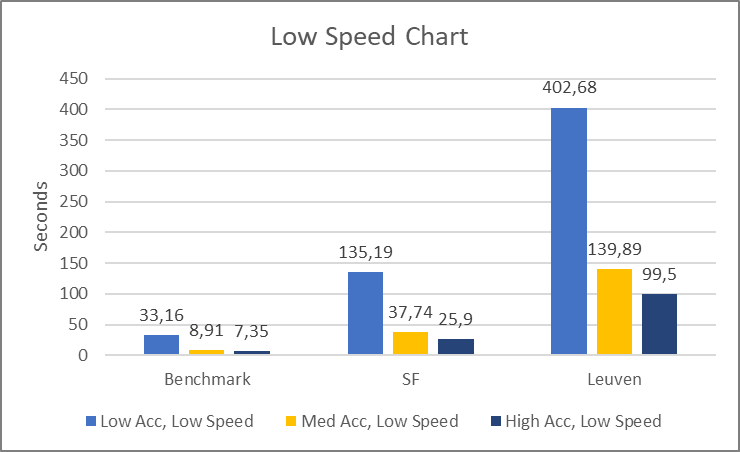
\includegraphics[width=\textwidth]{img/agility-low-speed}
        		\caption{The effects of a varying maximum acceleration and a low maximum velocity.}
        		\label{fig:agility-low-speed}
	\end{subfigure}
		
	\begin{subfigure}[t]{.9\textwidth}
        		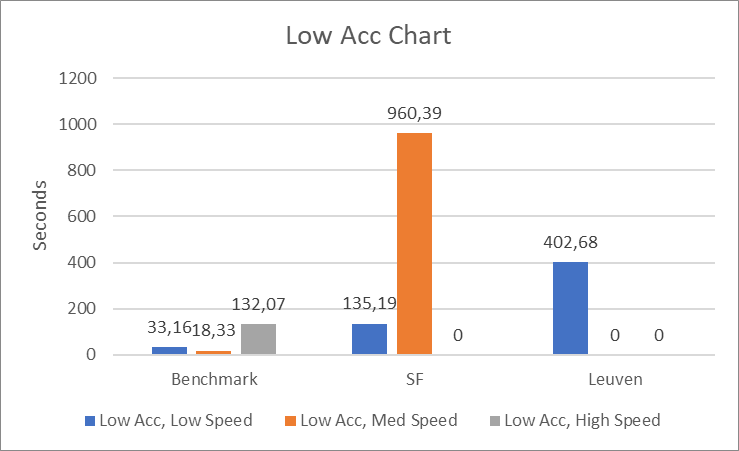
\includegraphics[width=\textwidth]{img/agility-low-acc}
        		\caption{The effects of a varying maximum velocity and a low maximum acceleration.}
        		\label{fig:agility-low-acc}
	\end{subfigure}	
	
        
    \caption{}\label{fig:agility-low}
\end{figure}

\begin{figure}
	\centering
	
	\begin{subfigure}[t]{.9\textwidth}
        		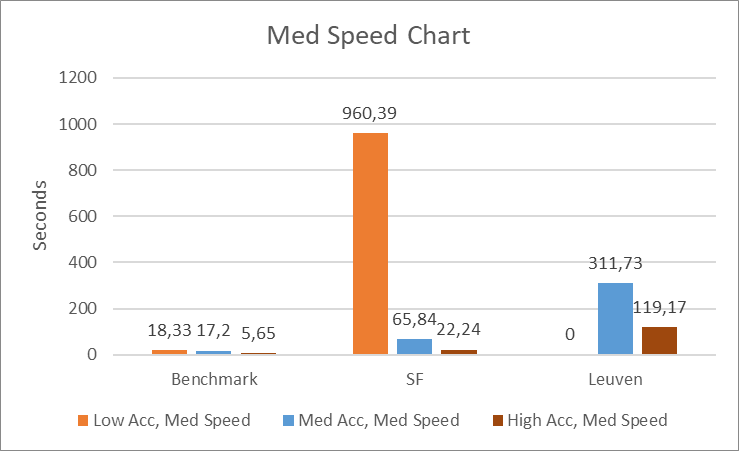
\includegraphics[width=\textwidth]{img/agility-med-speed}
        		\caption{The effects of a varying maximum acceleration and a medium maximum velocity.}
        		\label{fig:agility-med-speed}
	\end{subfigure}
		
	\begin{subfigure}[t]{.9\textwidth}
        		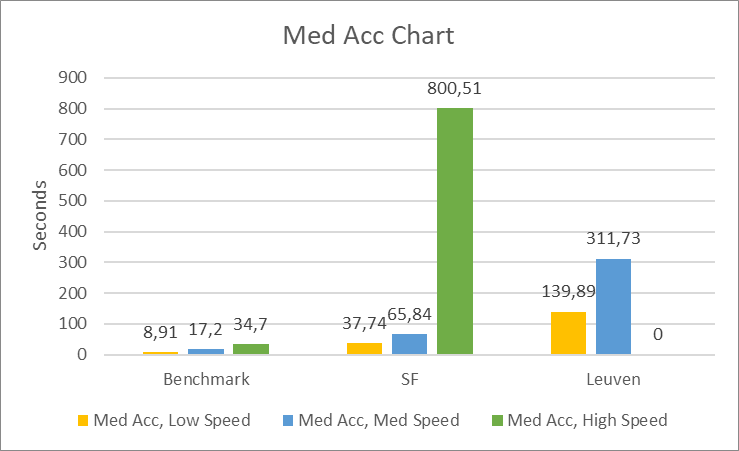
\includegraphics[width=\textwidth]{img/agility-med-acc}
        		\caption{The effects of a varying maximum velocity and a medium maximum acceleration.}
        		\label{fig:agility-med-acc}
	\end{subfigure}	
	
        
    \caption{}\label{fig:agility-med}
\end{figure}

\begin{figure}
	\centering
	
	\begin{subfigure}[t]{.9\textwidth}
        		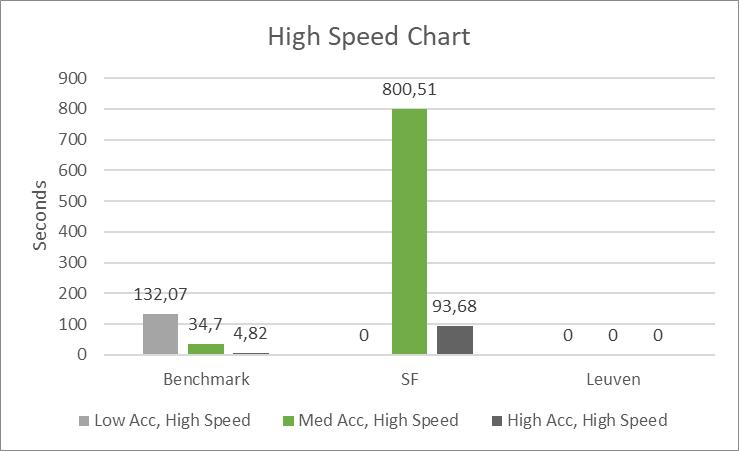
\includegraphics[width=\textwidth]{img/agility-high-speed}
        		\caption{The effects of a varying maximum acceleration and a high maximum velocity.}
        		\label{fig:agility-high-speed}
	\end{subfigure}
		
	\begin{subfigure}[t]{.9\textwidth}
        		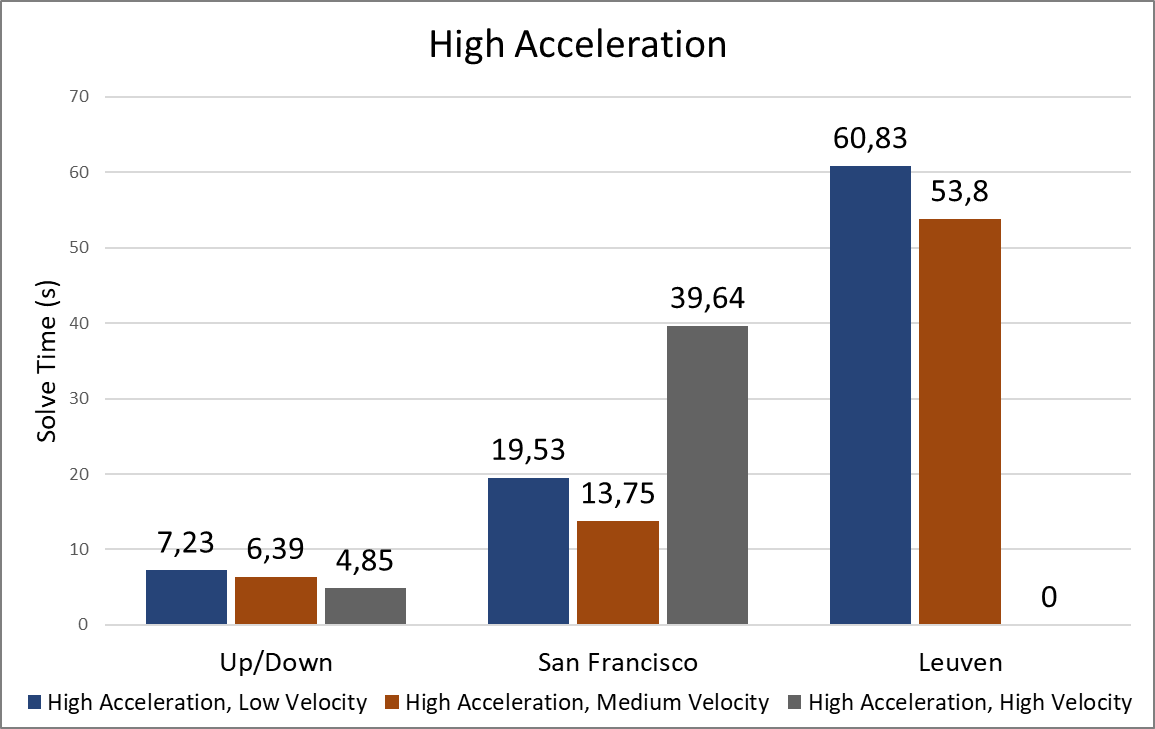
\includegraphics[width=\textwidth]{img/agility-high-acc}
        		\caption{The effects of a varying maximum velocity and a high maximum acceleration.}
        		\label{fig:agility-high-acc}
	\end{subfigure}	
	
        
    \caption{}\label{fig:agility-high}
\end{figure}



\clearpage
\section{Stability}
\label{subsec:stability}
\begin{figure}[]
	\centering
	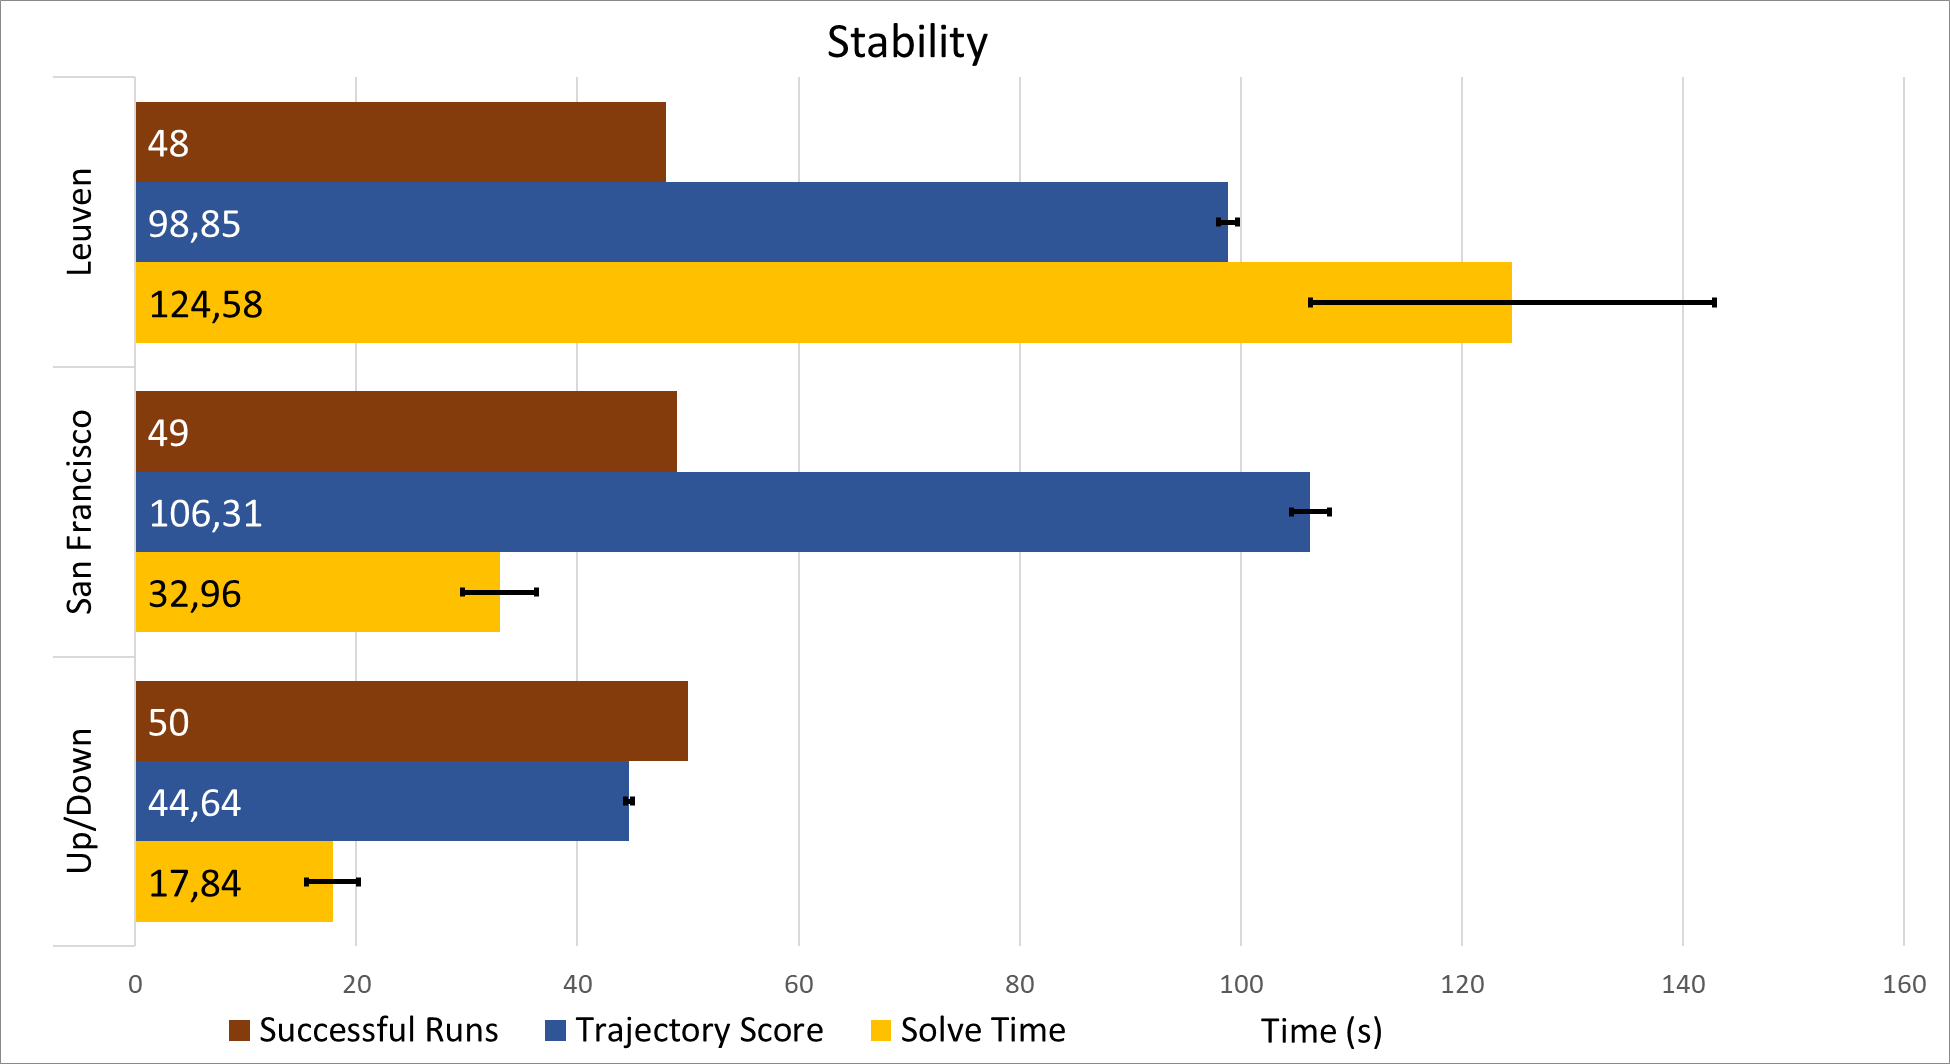
\includegraphics[width=\textwidth]{stability-data}
	\caption{stability data}
	\label{fig:stability-data}
\end{figure}
Stability is an important property of an algorithm. When the same problem is solved several times, the algorithm should not occasionally fail to solve the problem or require a wildly different amount of time to solve that problem. \\
This experiment aims to measure the stability of the algorithm. Each of the testing scenarios is executed 50 times, instead of 5 like in the other tests. Figure \ref{fig:stability-data} shows the results of this test. The error bars show sample standard deviation. \\

\subsection{Interpretation}
Even though the each sub-problem should ensure that the next segment can be solved, occasionally this was not the case as demonstrated in Figure \ref{fig:transition-fail}. It seems like a collision is inevitable, but that is actually not the case as demonstrated in \ref{fig:leuven-fail}. I believe this may be a bug in how the algorithm transitions between segments. I could not properly figure out what cases this bug in time.
\par
However, the algorithm does find a good trajectory in nearly all cases. When it does succeed, the variation in trajectory score is minimal. The solve time variation is also low, although it is a significantly higher for the Leuven scenario than for the others.
\begin{figure}[]
	\centering
	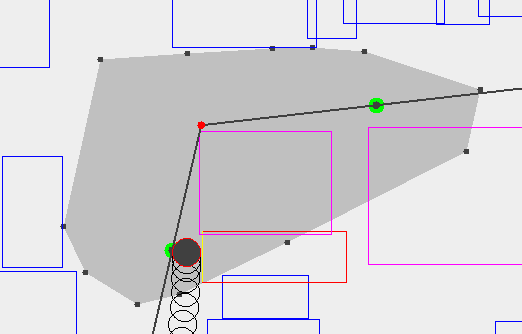
\includegraphics[width=0.5\textwidth]{transition-fail}
	\caption{A case where the transition between segments fails}
	\label{fig:transition-fail}
\end{figure}

\begin{figure}
	\centering
	
	\begin{subfigure}[t]{.45\textwidth}
        		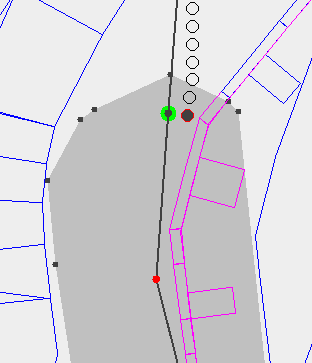
\includegraphics[width=\textwidth]{img/leuven-fail-pre}
        		\caption{This segment starts and fails with what seems like an inevitable collision...}
        		\label{fig:leuven-fail-pre}
	\end{subfigure}
	\hfill
	\begin{subfigure}[t]{.45\textwidth}
        		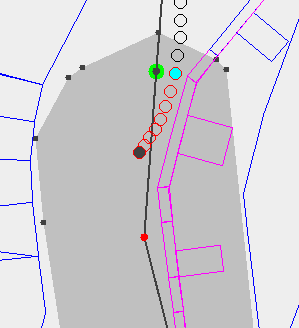
\includegraphics[width=\textwidth]{img/leuven-fail-post}
        		\caption{... However, this shows the trajectory in the previous segment after the goal in that segment has been reached in red. Clearly a collision is not inevitable.}
        		\label{fig:leuven-fail-post}
	\end{subfigure}	
	
        
    \caption{}\label{fig:leuven-fail}
\end{figure}



\clearpage
\section{Cornercutting}
\label{subsec:cutting}
A trajectory that allows corner cutting cannot be considered safe. However, additional constraints are required to prevent this from happening. This experiment attempts to measure the impact of the corner cutting prevention. The scenarios are solved with the corner cutting mitigation from section \ref{subsec:corner-cutting} both enabled and disabled. Figure \ref{fig:corner-data} shows the results. 

\begin{figure}[]
	\centering
	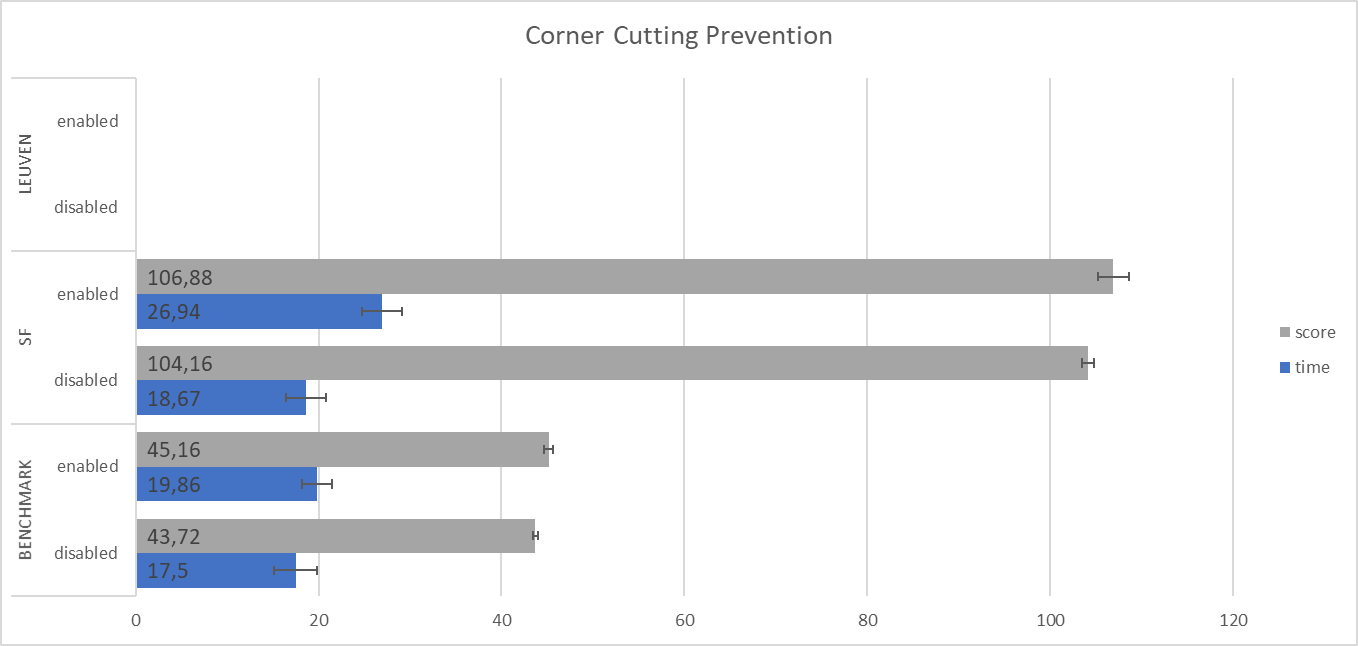
\includegraphics[width=\textwidth]{corner-cutting-data}
	\caption{The error bars show the 95\% confidence interval.}
	\label{fig:corner-data}
\end{figure}

\subsection{Interpretation}
As expected, enabling the corner cutting prevention has a negative impact on performance. This effect is limited for the Up/Down and San  Francisco scenarios. For the Leuven Scenario, the solve time more than doubles. This is likely due to the higher obstacle density and complexity.


\clearpage
\section{Linear approximation}
\label{subsec:lin-approx}
The velocity and acceleration of the UAV are limited to some finite value. Because both of those quantities are vectors, that maximum can only be approximated with linear constraints. More constraints are needed to model this more accurately which can allow for faster solutions. However, more constraints also have a performance cost. This experiment analyses the trade-off that needs to be made. The amount of vertices used for the linear approximation is tested with values of 6, 12 and 24.
\begin{figure}[]
	\centering
	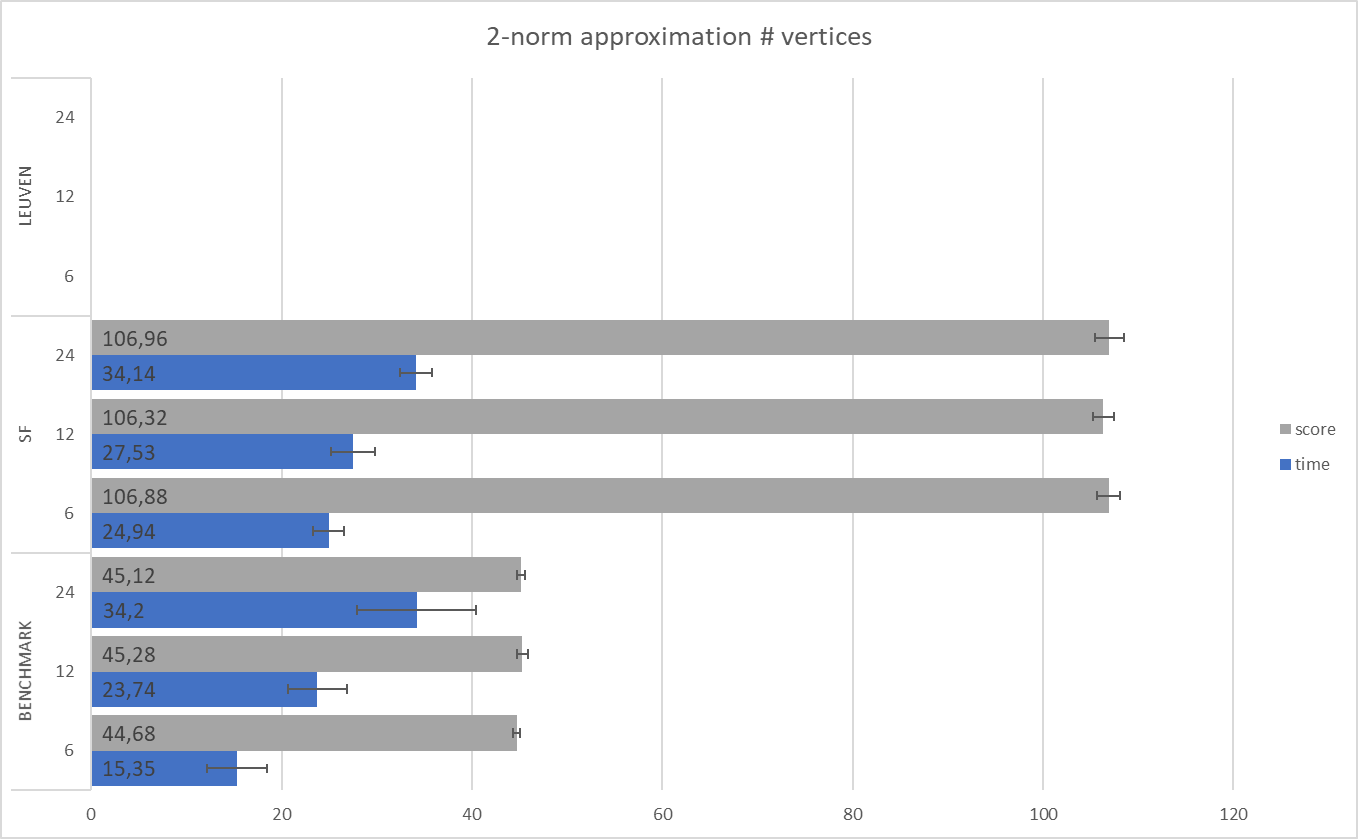
\includegraphics[width=\textwidth]{linear-data}
	\caption{linear approx data}
	\label{fig:linear-approx-data}
\end{figure}



\subsection{Interpretation}
In all cases, increasing the amount of vertices used to approximate the 2-norm also increases the solve time. The effect on trajectory score seems to be minimal for the Up/Down and Leuven trajectory. However, for the San Francisco trajectory there is a noticeable improvement with the better approximation.

\clearpage
\section{Time step size}
\label{subsec:timestep}
The time step size determines how many time steps are used in each MILP problem. The discretized time steps are samples at regular intervals of the continuous trajectory that the UAV would actually travel in the real world. As a result, the trajectory defined by those time steps is a piece-wise linear approximation of this smooth, real world trajectory. \\
As the size of each step goes to zero, the approximation becomes more accurate. This also means that the trajectory should become faster, since the UAV can be controlled more precisely through time. This allows for more aggressive maneuvers. \\
However, adding more time steps increases the amount of integer variables and constraints. This comes at a performance cost. \\
In this experiment, three different time step sizes are tested. The $0.2s$ default value, as well as $0.1s$ and $0.5s$ are tested.
\begin{figure}[]
	\centering
	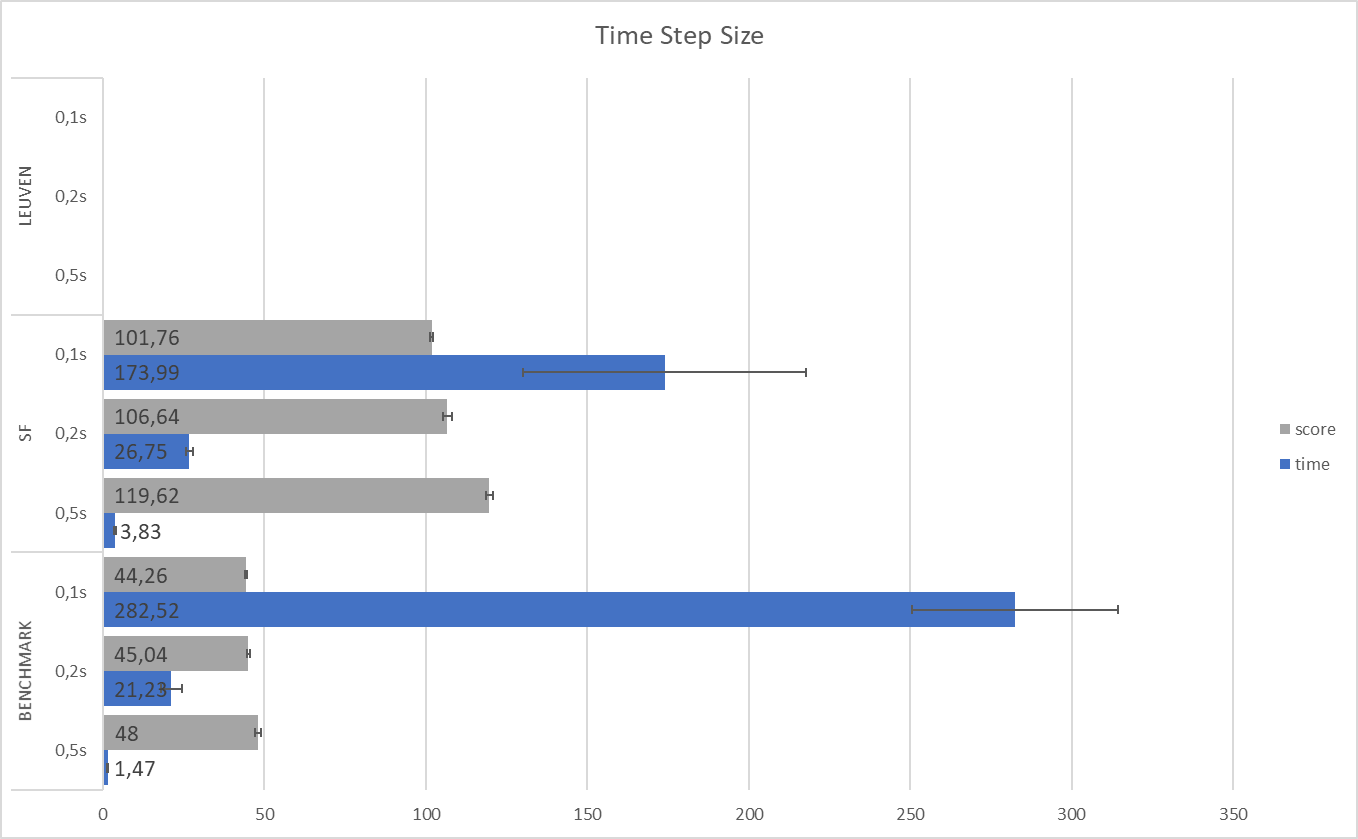
\includegraphics[width=\textwidth]{timestep-data}
	\caption{time step data}
	\label{fig:timestep-data}
\end{figure}
\subsection{Interpretation}
The time step size has a dramatic impact on performance. Changing the time step size from $0.2s$ to $0.1s$ or $0.5s$ changes the solve time by a factor of 5 to 10 or even more for the Up/Down scenario. This experiment really shows the exponential complexity of MILP. Making the time steps smaller makes the algorithm much slower.
\par
As expected, decreasing the time step size also improves the score of the trajectory. The largest gain is the step from $0.5s$ to $0.2s$, although there still is some improvement when going to $0.1s$.

\clearpage
\section{Max Time}
\label{subsec:maxtime}
\begin{figure}[]
	\centering
	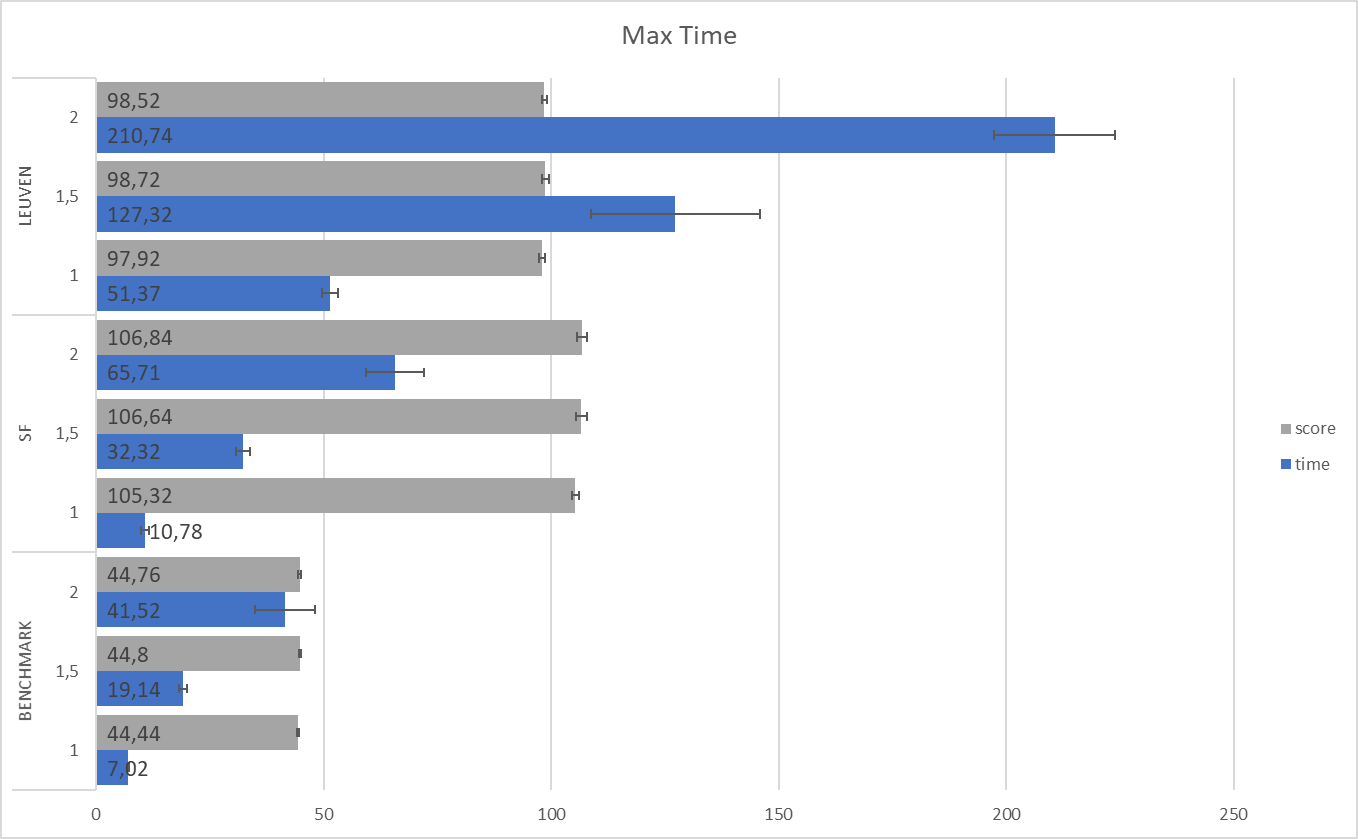
\includegraphics[width=\textwidth]{maxtime-data}
	\caption{maxtime data}
	\label{fig:maxtime-data}
\end{figure}
For each sub-problem, the amount of time steps to model needs to be determined in advance. The algorithm calculates an estimated upper bound for the time (and thus the amount of time steps). In the ideal case, this upper bound is equal to the time needed for the optimal trajectory. However, if the upper bound is too low, no solution can be found.\\
This experiment looks at the importance of a low upper bound on the time needed. By default, the estimated upper bound is multiplier by 1.5 to ensure enough time steps are available. A multiplier of 1 is also tested, along with a multiplier of 2. 

\subsection{Interpretation}
The time needed to solve the scenarios is heavily influenced by maximum time given. For these scenarios, the default multiplier of 1.5 seems unnecessary and could be lowered to 1 without issues. Increasing the multiplier to 2 nearly doubles the solve time across the board.


\clearpage
\section{Approach Margin}
\label{subsec:approach-margin}
\begin{figure}[]
	\centering
	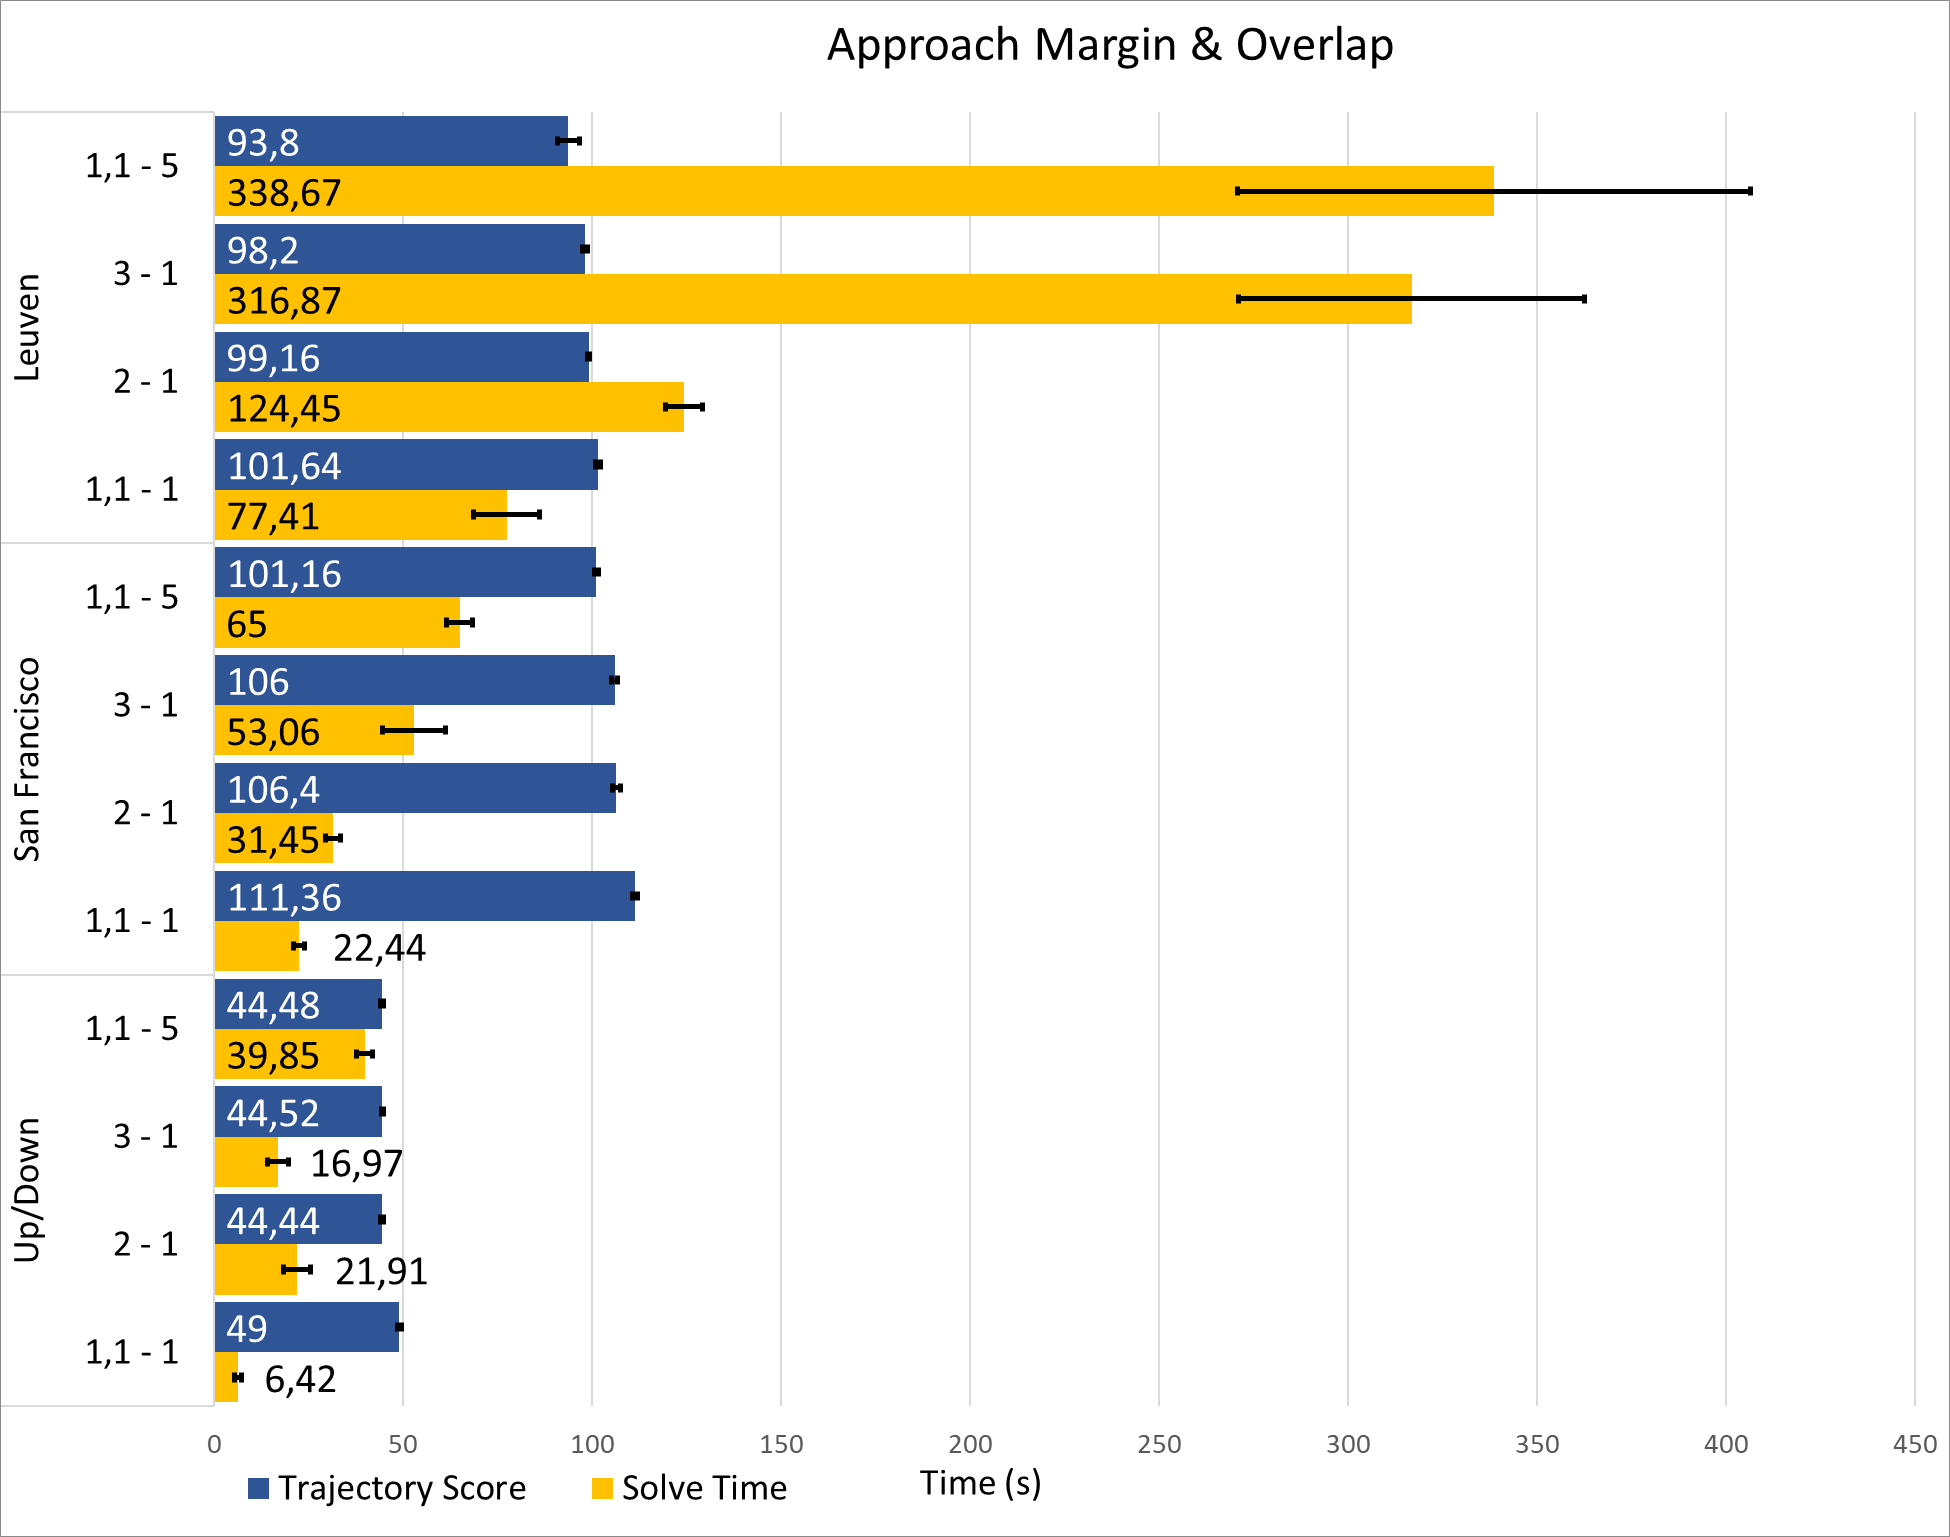
\includegraphics[width=\textwidth]{approach-data}
	\caption{approach data}
	\label{fig:approach-data}
\end{figure}
TODO

\subsection{Interpretation}
TODO

\clearpage
\section{Genetic Algorithm Parameters}
\label{subsec:ga-params}
TODO



\newpage


\chapter{Discussion}
The goal of this thesis is build a scalable approach for MILP trajectory planning. The target vehicles are multirotor UAVs, so the results in the previous section need to be analyzed in that context. \\
The first step is analyzing whether or not the approach is actually scalable enough when planning the trajectory for this kind of vehicle through complex environments.\\
Afterwards, the other experiments demonstrate the importance of some of the parameters used in the algorithm. The results provide insight in the limitations of the current approach, and how it may be improved in the future.

\section{Research question result}


The general performance results show that the algorithm is capable of planning a long trajectory through complex environments. Even for the smallest scenarios, the solver struggles to find a trajectory without preprocessing. With my algorithm, the UAV can successfully navigate an entire city. \\
The convexity test demonstrates that convexity of the search space is indeed a large factor. This supports the assumption that my entire algorithm is built upon: Maintaining convexity as much as possible is required to make the algorithm scale. \\
The stability test shows that, for the most part, my segmentation approach preserves stability. There still are some issues around the transitions between segments, but they can be eliminated by slightly overlapping the segments. This overlap comes at a performance cost, but it also improves the quality of the trajectory. Overall I am not entirely satisfied with the stability of my current implementation, however I do believe the small issues around segment transitions can be resolved. \\\\

The results show a large improvement in scalability in certain realistic scenarios, but the choice of those scenarios has drastically impacted the algorithm I have developed.\\

During development, I have always used realistic approximations of the capabilities of multirotor UAVs. Those can reach high accelerations but have relatively low maximum velocities compared to what fixed-wing aircraft can achieve. This makes those vehicles very agile, which is one of the contributing factors to their recent popularity. \\
The assumption of this agility means that my algorithm cannot be applied to UAVs which do not have that property. One of the properties my algorithm uses often is the maximum acceleration distance, which is the distance in which the UAV can always come to a complete stop. This works fine with multirotor UAVs, but is a meaningless concept when dealing with fixed-wing UAVs which cannot stop at all during flight. \\
However, those kinds of low-agility UAVs are unlikely to be deployed at low altitudes in dense city centers exactly because they lack agility. Even with perfect planning, cities are very unpredictable places. An multirotor UAV is much more likely to be able to safely react to an unexpected obstacle than a fixed-wing UAV. \\
While I picked out fixed-wing UAVs as an example, the same arguments hold for any kind of UAV that either cannot hover or has low agility. Some UAVs may be able to hover, but are not very agile due to a high maximum velocity and low acceleration. In this case, the agility can be improved by reducing the maximum velocity.\\ \\

The density of obstacles is also an extremely important factor. The Leuven scenario is significantly harder than the San Francisco scenario because the obstacles are smaller and closer together. Not only are the obstacles closer together, but they are also polygons and can have many more edges per obstacle. For scenarios where the obstacles are significantly denser or complex than in the Leuven scenario, the approach may not improve the performance enough. \\
On the other hand, the Leuven map is much more detailed than is required for navigation. Many obstacles could be merged together without a significant on possible trajectories. The obstacles could also be simplified, reducing the amount of edges per obstacle. Given that the Leuven map is unprocessed except for calculating the convex hull of each obstacle, the algorithm should be able to handle most real world maps when properly prepared.

Given these considerations, I conclude that my approach meets the basic requirements. The assumptions behind the design of the algorithm seem to be valid based on experiments.

\section{Factors}
While the chosen parameter values allow the algorithm to scale well, different values may be chosen to find a different balance between performance and solution quality. \\
The corner cutting prevention makes the trajectory slightly slower, but that is to be expected since cutting a corner is faster than going around. The performance does take a hit, but the extent is minimal. The corner cutting prevention constraints seem certainly worth being enabled. \\
The 2-norm approximation has a slightly larger effect on performance. However, there does not seem to be an impact on the trajectory speed. This value could be reduced for a small performance gain. \\ \\

The time step size and maximum time both have a dramatic impact on the performance. The time step size should be no smaller than necessary, and the maximum time should be as small as possible. They are by far the most important performance factors. As a result, further improvements on performance should focus on these factors. A way to improve performance may be solving each segment twice: Once with a high time step size and a conservative maximum time, and another time with a smaller time step size and a very tight maximum time. The first run quickly and provides a tight upper limit on the amount of time needed for the segment. The second run would also run significantly faster, since the amount of time steps modeled is much closer to what is actually needed. Due to a lack of time, I was unable to implement this. \\

The approach margin data is probably the strangest. Going from a low to medium approach margin increases the solve time and improves the trajectory, as expected. However, increasing the approach margin again actually decreases the solve time again, as well as reducing the quality of the trajectory. This is unexpected since a approach margin should lead to larger segments which take longer to solve. The larger segments should also improve the quality of the solution because corners can be taken more efficiently, yet the the opposite happens in the data. TODO: find answer?






%\subsection{evolution of understanding}
%One of the main recurring patterns in my thesis is the concept of convexity. Early on in the thesis I was not aware of the importance of convexity. The worst case performance of MILP depends on the amount of integer variables, so my early attempts at improving performance were focused on reducing the amount of integer variables. \\
%Segmenting the trajectory planning problem into smaller pieces was part of that effort to reduce the amount of integer variables. However, at the time I was not aware of the relation between turns and convexity. I decided to focus on the turns from a purely pragmatic stand point. Each turn is a maneuver. To find the optimal trajectory for that maneuver, the maneuver should be solved in a single segment. Based on this idea, the core of my algorithm was built. \\
%This was functional by the end of the first semester. By this time, I had figured out that obstacles necessarily cause a non-convex search space. I used this insight to separate obstacles on the inside of turns from those on the outside. The algorithm produced promising results, but I did not fully understand ....TODO?
%
%However, the algorithm only supported grid aligned rectangles for obstacles with the San Francisco dataset. To really test the algorithm, it needed to support  arbitrary polygons as obstacles. Implementing this caused many small and large problems. There were many implicit assumptions that worked with the grid-aligned rectangles. I also ran into scaling issues with my preprocessing algorithm.

\section{Critical Review}